%%%%%%%%%%%%%%%%%%%%%%%%%%%%%%%% 
\section{The Charge Readout System} 
\label{sec:detectors-fd-alt-chg-readout}

In the %liquid-gas 
dual-phase LArTPC concept, the ionization charge is first
extracted into the argon gas phase by an extraction grid (stainless steel
wires tensioned in both $x$ and $y$ directions) using a 2-kV/cm electric field of. %around . \fixme{Something about the extr grid}
%
The charge is amplified by a Large
Electron Multiplier (LEM). A LEM, with a 30-kV/cm field across its electrodes,
works by triggering Townsend multiplication in
the high electric field regions (called LEM holes) within its micro pattern inner structure~\cite{Bondar:2008yw}. 
%
The amplified charge is then collected and recorded on a
2D anode consisting of a set \fixme{two sets?} of 3.125-mm-pitch strips 
that provide the $x$ and $y$ coordinates (and thus two views) of the event. 

Typical electric fields between each
stage of the readout are illustrated in Figure~\ref{fig:setup}. Table~\ref{tab:crp_dist}
shows the inter-stage distance and the tolerances required to obtain 
uniformity of gain to within $\sim$5\%.
\begin{cdrfigure}[Dual-phase readout]{setup}{Illustration of the electric fields in the amplification region of a dual-phase LArTPC. The simulated field lines in dark blue indicate the paths followed by the drifting charges (without diffusion).}
 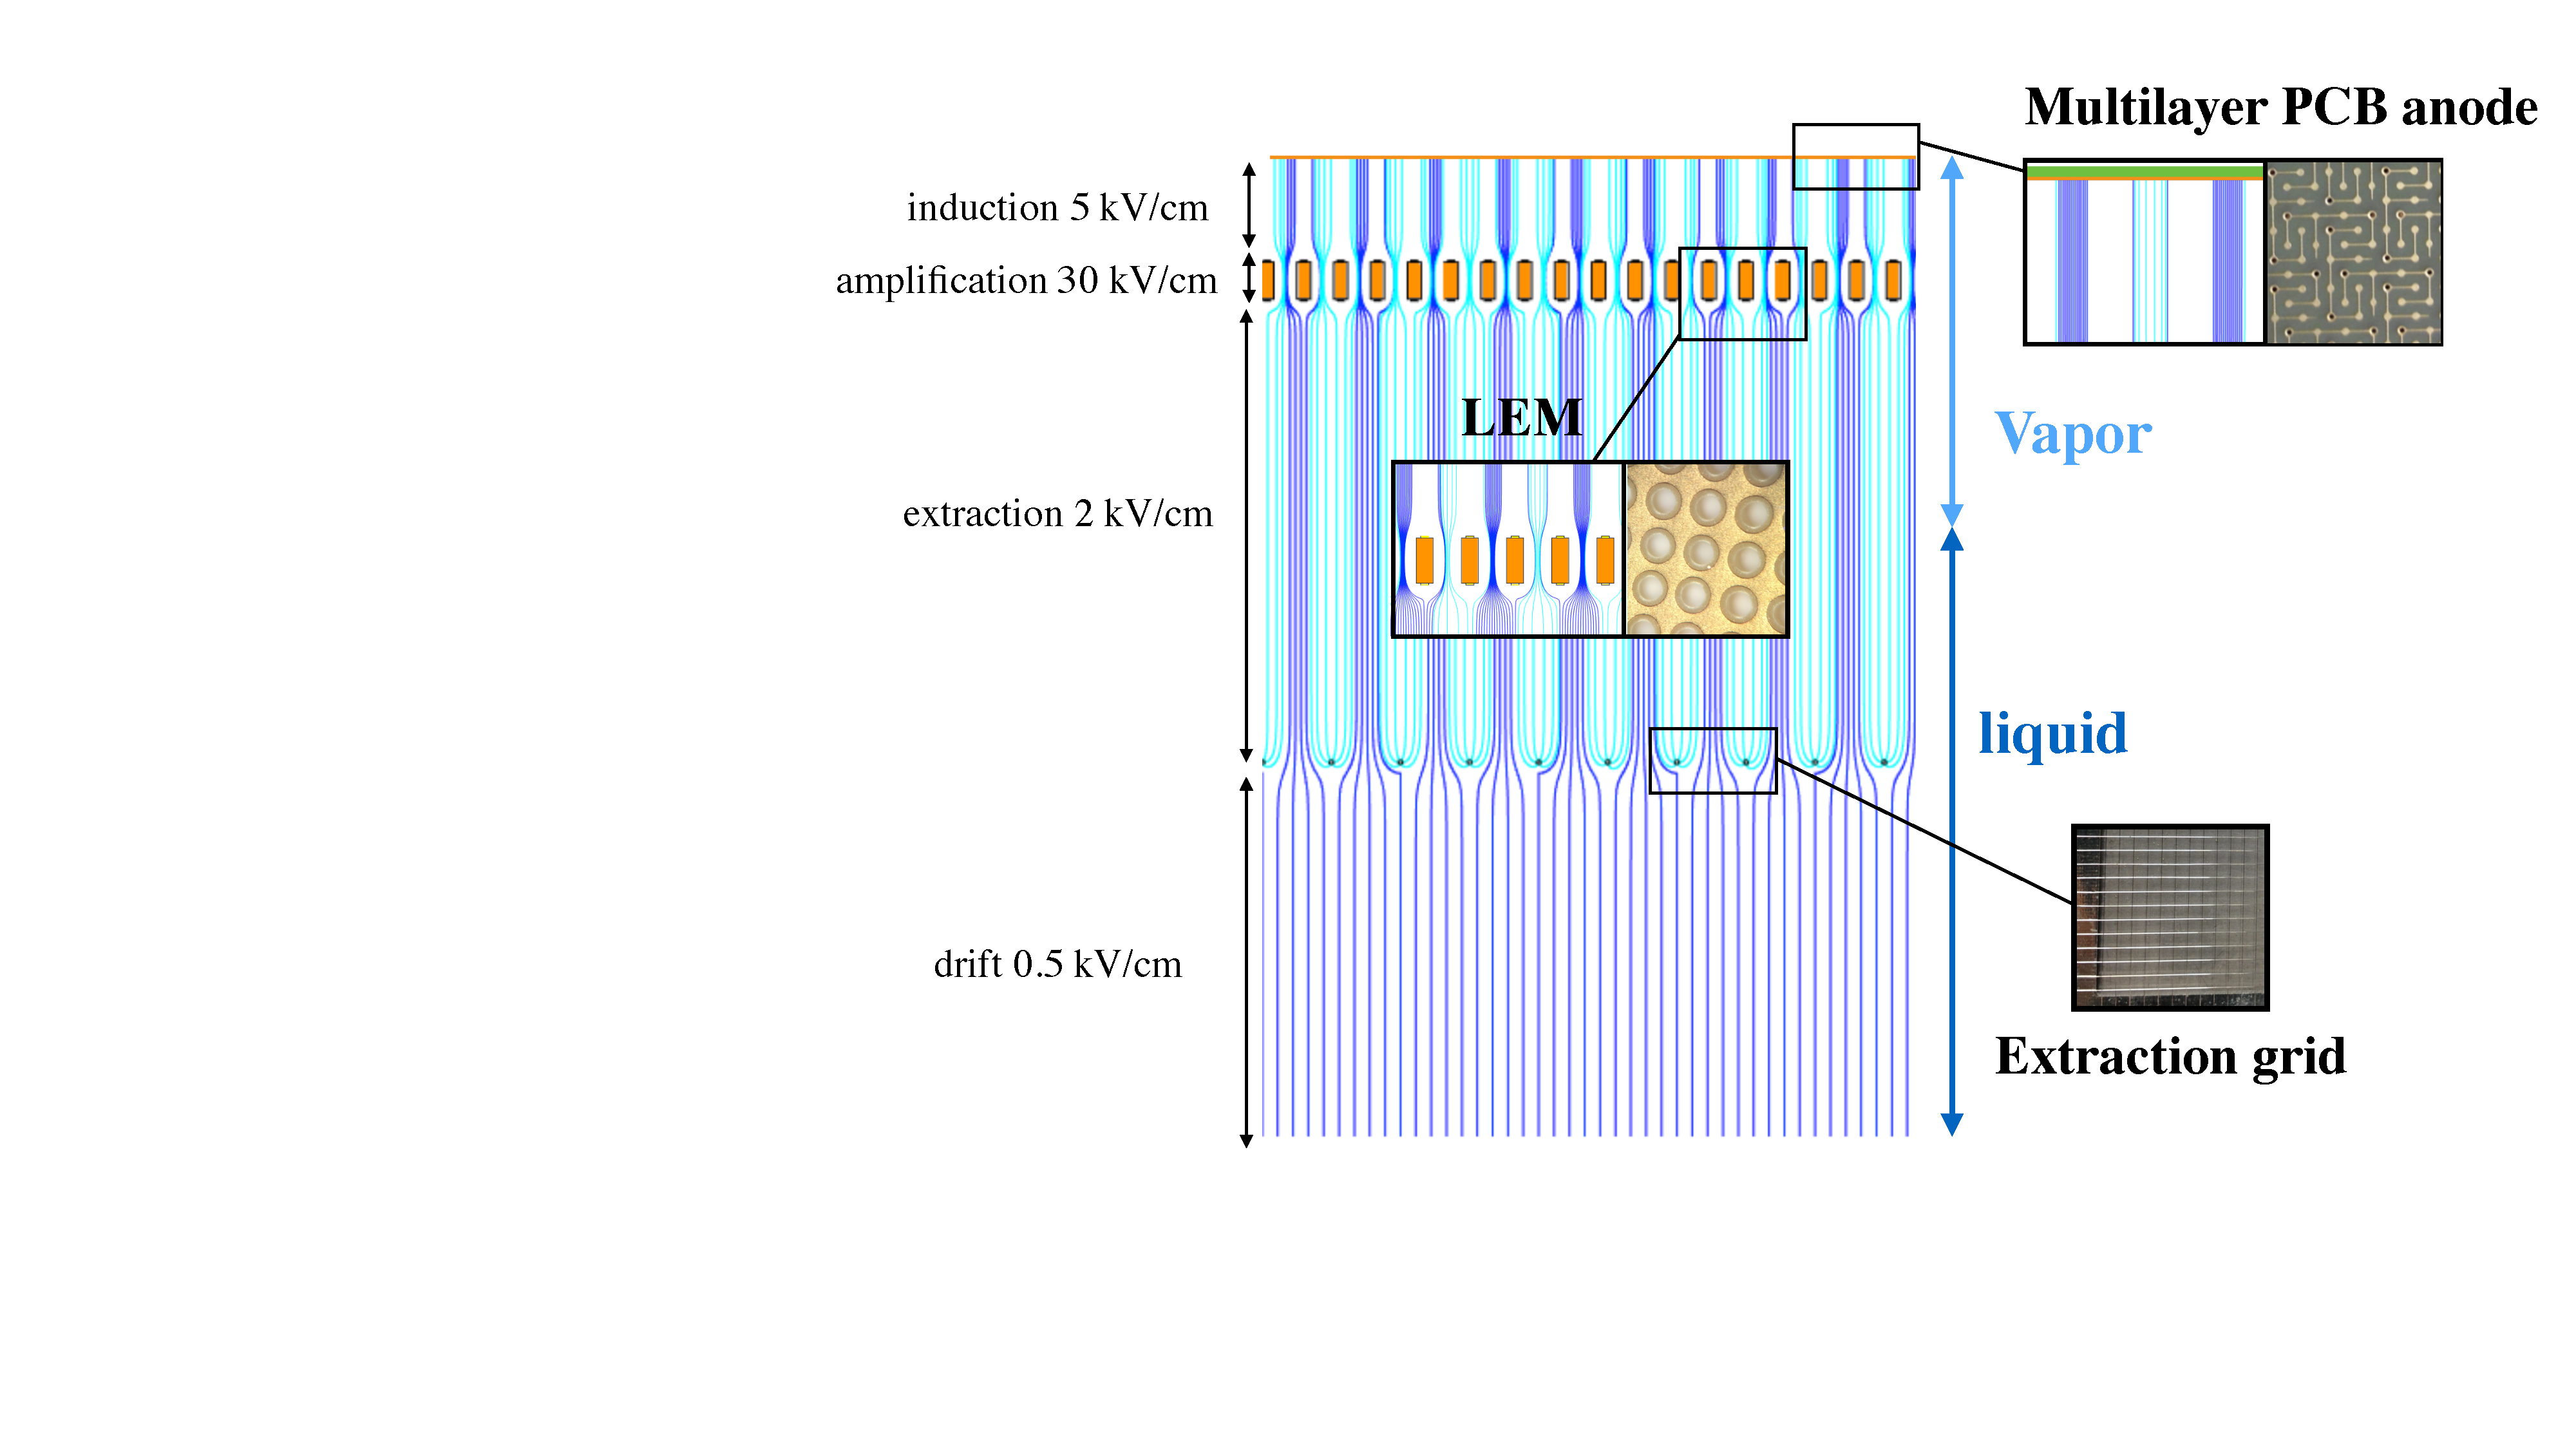
\includegraphics[width=.8\textwidth]{double_phase_principle.pdf}  
\end{cdrfigure}
\begin{cdrtable}[Interstage distances and electric field settings of the dual-phase readout components]{lp{2cm}p{2cm}l}{crp_dist}{Interstage distances and electric field settings of the dual-phase readout components.} 
 Component & Distance [mm] & Tolerance [mm] & Electric field [kV/cm]  \\ \toprowrule
 Anode-LEM top electrode  & 2 & 0.1 & 5\\ \colhline
 LEM top-bottom electrode   & 1 & 0.01 & 30-35\\ \colhline
 LEM bottom electrode-grid        & 10 & 1 & 2 (in LAr) and 3 (in GAr)\\
 \end{cdrtable}

The three stages (extraction grid, LEM and anode) are assembled into multi-layered,
sandwich-like modular units (\num{9}m$^2$ in area) with precisely
defined inter-stage distances and inter-alignment; these modular units are called Charge
Readout Planes (CRPs). \fixme{contrast CRP with LAS, defined in next section}
   
\subsection{The Charge Readout Plane (CRP)}

Each CRP is an independent detector element that performs charge extraction, multiplication and
collection, and has its own high voltage system and independent signal feedthroughs. The entire area of the LEM and anode in a CRP is active.
% size
The LBNO 20-kt detector design (described in \anxlbnob) featured
modularized CRPs of dimensions of 4$\times$4~m$^2$, with 2-m long strips. For the DUNE cryostat
geometry, a size of 3$\times$3~m$^2$ with a strip length of 3~m is found to be optimal.
%
%The design and the functional concept of the CRP are exactly the same in the two cases, however the length of the strips is 2~m for the 4$\times$4~m$^2$ CRPs and 3~m for the 3$\times$3~m$^2$ CRPs.
%
  The description in this section is based on
the LBNO 4$\times$4~m$^2$ CRP.  

% composition
LEM and anode units of
$50\times50$ cm$^2$, called LEM/Anode Sandwich (LAS) modules, are assembled into a CRP.
\fixme{what's the difference between a LAS and a CRP, the extraction grid? This is confusing}
The adjacent anodes are bridged together to
form readout strips of the required length by connecting short flat
cables to KEL connectors 
\fixme{write out what KEL stands for} soldered on their top side. The signals from
the last anode 
\fixme{The anode strip at the edge? I can't picture the ``last'' one}
are brought to the front-end electronics embedded
within dedicated signal-feedthrough chimneys. \fixme{are chimneys just pipes for things to go through?}
% installation
Each CRP is
independently hung from the vessel deck through its three suspension
feedthroughs. 
% composition
%The CRP has its own high voltage system and its independent signal feedthroughs. 
%configuration
Figure~\ref{fig:4_4CRP_FRONT} illustrates the 4$\times$4 m$^2$ CRP; its characteristics
are summarized in Table~\ref{tab:crp_para}.

\begin{cdrfigure}[Side and top views of the $4\times4$~m$^2$ CRP]{4_4CRP_FRONT}{Side and top views of the $4\times4$~m$^2$ CRP designed for LBNO (units in mm).}
 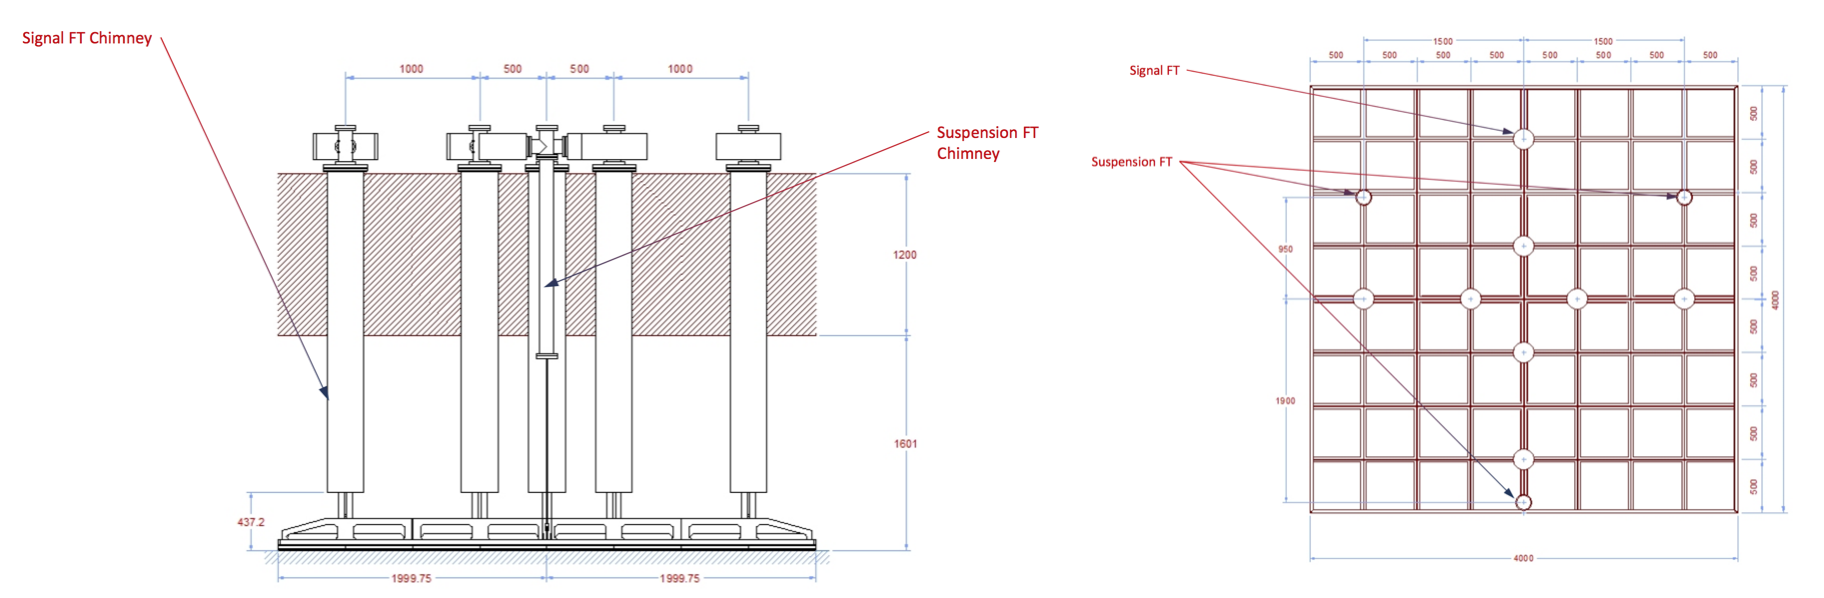
\includegraphics[width=\textwidth]{4_4_CRP_top-side-view}  
\end{cdrfigure}
\begin{cdrtable}[Numbers of components of the 4$\times$4 m$^2$ CRP]{lr}{crp_para}{Numbers of components of the 4$\times$4 m$^2$ CRP designed for LBNO} 
Component & Number \\ \toprowrule
$50\times50$ cm$^2$ anode panels & 64\\ \colhline
$50\times50$ cm$^2$ LEM  panels&  64\\ \colhline
Signal  feedthroughs & 8\\ \colhline
Suspension  feedthroughs & 3\\ \colhline
Readout strip length (m)& 2\\ \colhline
Number of channels & 5120\\
\end{cdrtable}

The entire area of the LEM and anode is active, as noted earlier, and each adjacent
$50\times50$~cm$^2$ LAS module \fixme{CRP?} has an inter-space \fixme{a gap?}
of only 0.5~mm. %It is therefore important to note that, 
Therefore, %although composed of independent LAS, 
the entire 4$\times$4~m$^2$ area of the
CRP is fully active, with a small gap every 50~cm that does not interfere with
the charge collection in the 3.125-mm readout pitch of the anode.

The extraction grid consists of 100~$\mu$m diameter stainless steel
wires tensioned in both $x$ and $y$ directions over the entire 4-m
length of the CRP. They are soldered into groups of 32 on independent
wire-tensioning pads %spaced 
oriented perpendicularly to the side of the CRP
frame. \fixme{needs good picture}
Each wire-tensioning pad consists of a printed circuit board (PCB) for HV-connection that is fixed to a
mechanical wire holder very precisely. The PCB %hosts the high voltage connection and
has 32 soldering pads with 200~$\mu$m grooves for precise positioning of
the wires. During the wire-soldering process each wire is tensioned by
150-g lead weights and positioned in a groove. 
(With this method LBNO achieved better than 50~$\mu$m precision on the wire pitch, measured under the microscope.)
%With this method the precision on the wire pitch, measured under the microscope, was better than 50~$\mu$m. The PCB is then fixed on the wire holder and the whole 
This system provides precise tension to the
group of 32 wires by pushing the holder against the CRP's FR4 frame. % with two stainless steel screws.

The 4$\times$4~m$^2$ CRP has 5120 readout channels
in total. It %The 4$\times$4~m$^2$ LBNO CRP is integrated with feedthroughs that perform different functions. 
The signals from the CRP are read out
through eight signal feedthroughs (SFTs) that host the front-end
electronics at its bottom and transmit the signal to the DAQ system
located on top outside of the vessel. \fixme{specify the anode-to-FE electronics connection}
  Each signal feedthrough groups
640 channels. %, and the 4$\times$4~m$^2$ CRP has 5120 readout channels in total.  
Three suspension feedthroughs are arranged as an
equilateral triangle whose barycenter coincides with that of the CRP; they suspend the CRP at the
required position and precisely adjust the CRP level with
respect to the liquid argon surface. Figure~\ref{fig:4_4CRP_3D} shows
a 3D view of this CRP, where the chimneys for
feedthroughs and the %$4\times4$~m$^2$ 
stiffening frame are visible.
\begin{cdrfigure}[3D view of the $4\times4$~m$^2$ CRP.]{4_4CRP_3D}{3D view of the $4\times4$~m$^2$ LBNO CRP.}
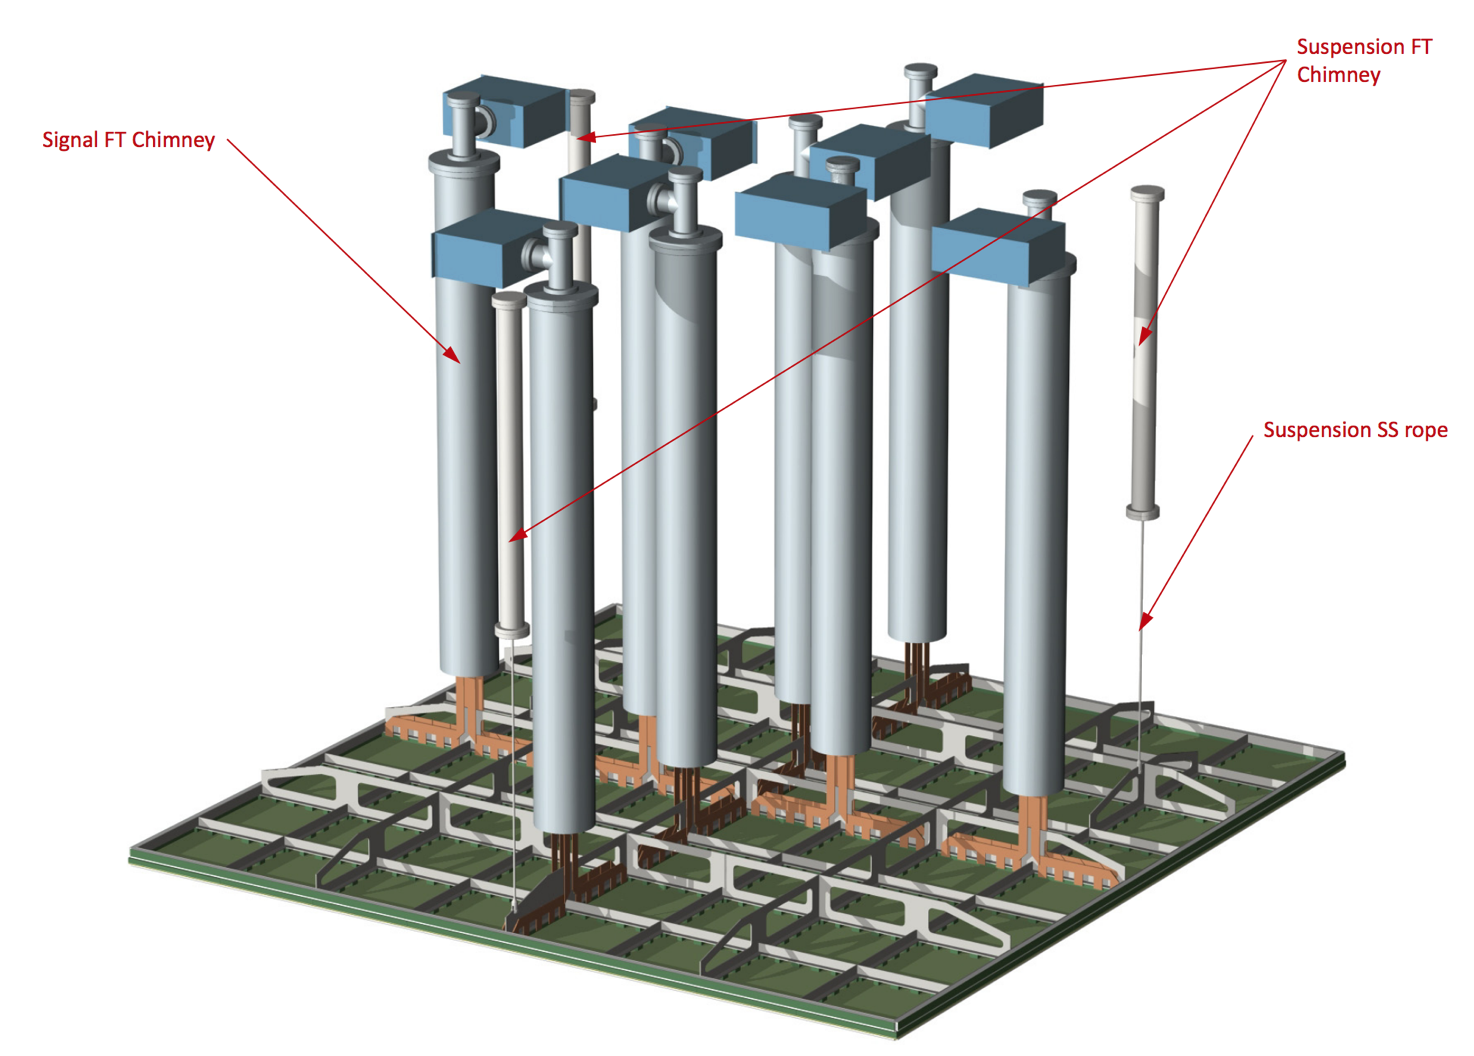
\includegraphics[width=0.8\textwidth]{4_4CRP_3D}  
\end{cdrfigure}

The $3\times3$~m$^2$ DUNE CRP %is a down-sized version of the LBNO one with dimensions of  and 3 
has three signal feedthrough chimneys and 1920 readout channels.

%%%%%%%%%%%%%%%%%%%%%%%%%%%%%%%%%%%%%%%%%
\subsection{The LEM/Anode Sandwich (LAS)}

LAS modules have been extensively studied as part of the ongoing CERN WA105
prototyping efforts (see~\ref{sec:proto-cern-double}). The LEMs and the anodes are produced by a PCB 
manufacturing company called ELTOS\footnote{\url{www.eltos.it}}. Their designs are the
outcome of intensive R\&D effort over the last few years, aimed at maximizing the S/N ratio %signal-to-noise ratio ($S/N$) 
for the large-area readouts foreseen for use in 
giant dual-phase LArTPCs.  Figure~\ref{fig:LEM_anode} shows the LEMs and anodes. %along with a zoom on their structure.
This section summarizes key features of the LAS.

\begin{cdrfigure}[Pictures of the LEM and anode along with microscope views]
{LEM_anode}{Top: pictures of the LEM and anode along with microscope
  views. Bottom: close up of the LEM HV connectors and back view of the anode 
with the KEL signal connectors to bridge to the adjacent LAS or to connect 
flat cables going to the signal feedthrough}
 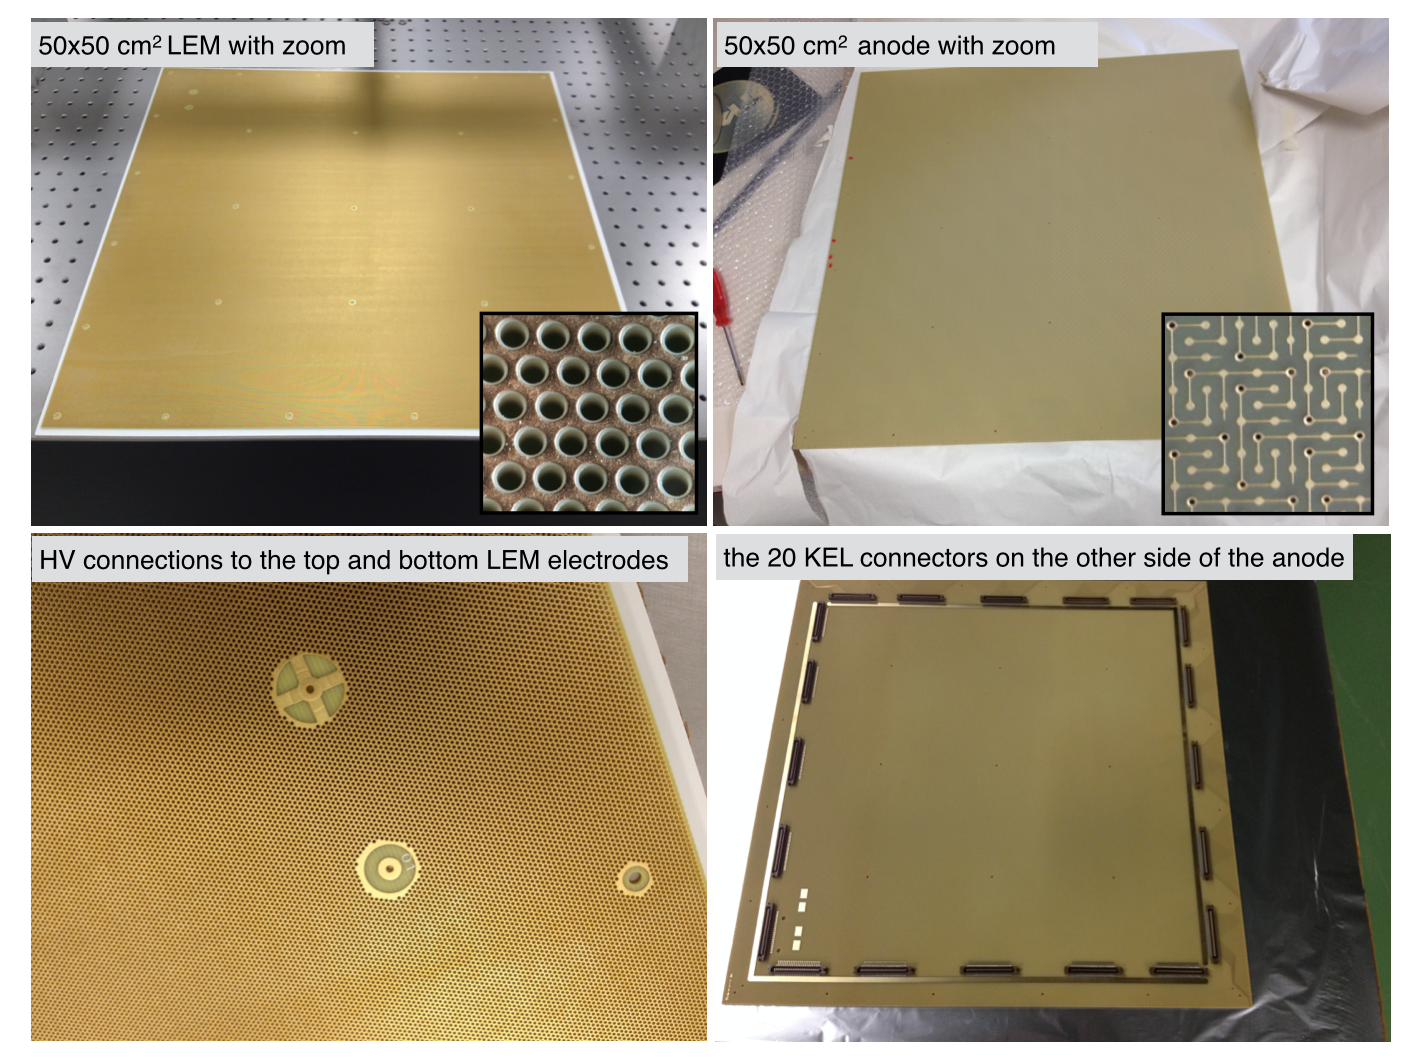
\includegraphics[width=.8\textwidth]{LEM_anode_zoom}  
 \end{cdrfigure}


 \paragraph{The 0.5$\times$0.5~m$^2$ anode:}
The anode is manufactured from a single multilayer Printed Circuit
Board (PCB). The readout strips for both $x$ and $y$ views  consist of
interconnected gold-plated copper tracks, corresponding %. The track pattern corresponds 
to the 3.125-mm readout pitch. The two views have
com-penetrating \fixme{what's com-penetrating?} track patterns that, however, are electrically
insulated by ensuring the crossing connections of the tracks on the
bottom layer of the PCB with a system of vias. \fixme{I cannot parse prev sentence} 
The design of the track
patterns is such that both $x$ and $y$ views collect the same amount
of charge, independent of the angle of charged-particle tracks with
respect to the readout strip orientation. This design has been
optimized by testing various PCB layouts %for the implementation of the readout strips 
as described in~\cite{Cantini:2013yba}.  The layout and
schematic of the anode are shown in Figure~\ref{fig:anode_sch}.

\begin{cdrfigure}[The 2D anode]{anode_sch}
{The 2D anode (left) and its schematic explaining the  interconnections 
between both views (right). One view is filled  in red and the other in white.}
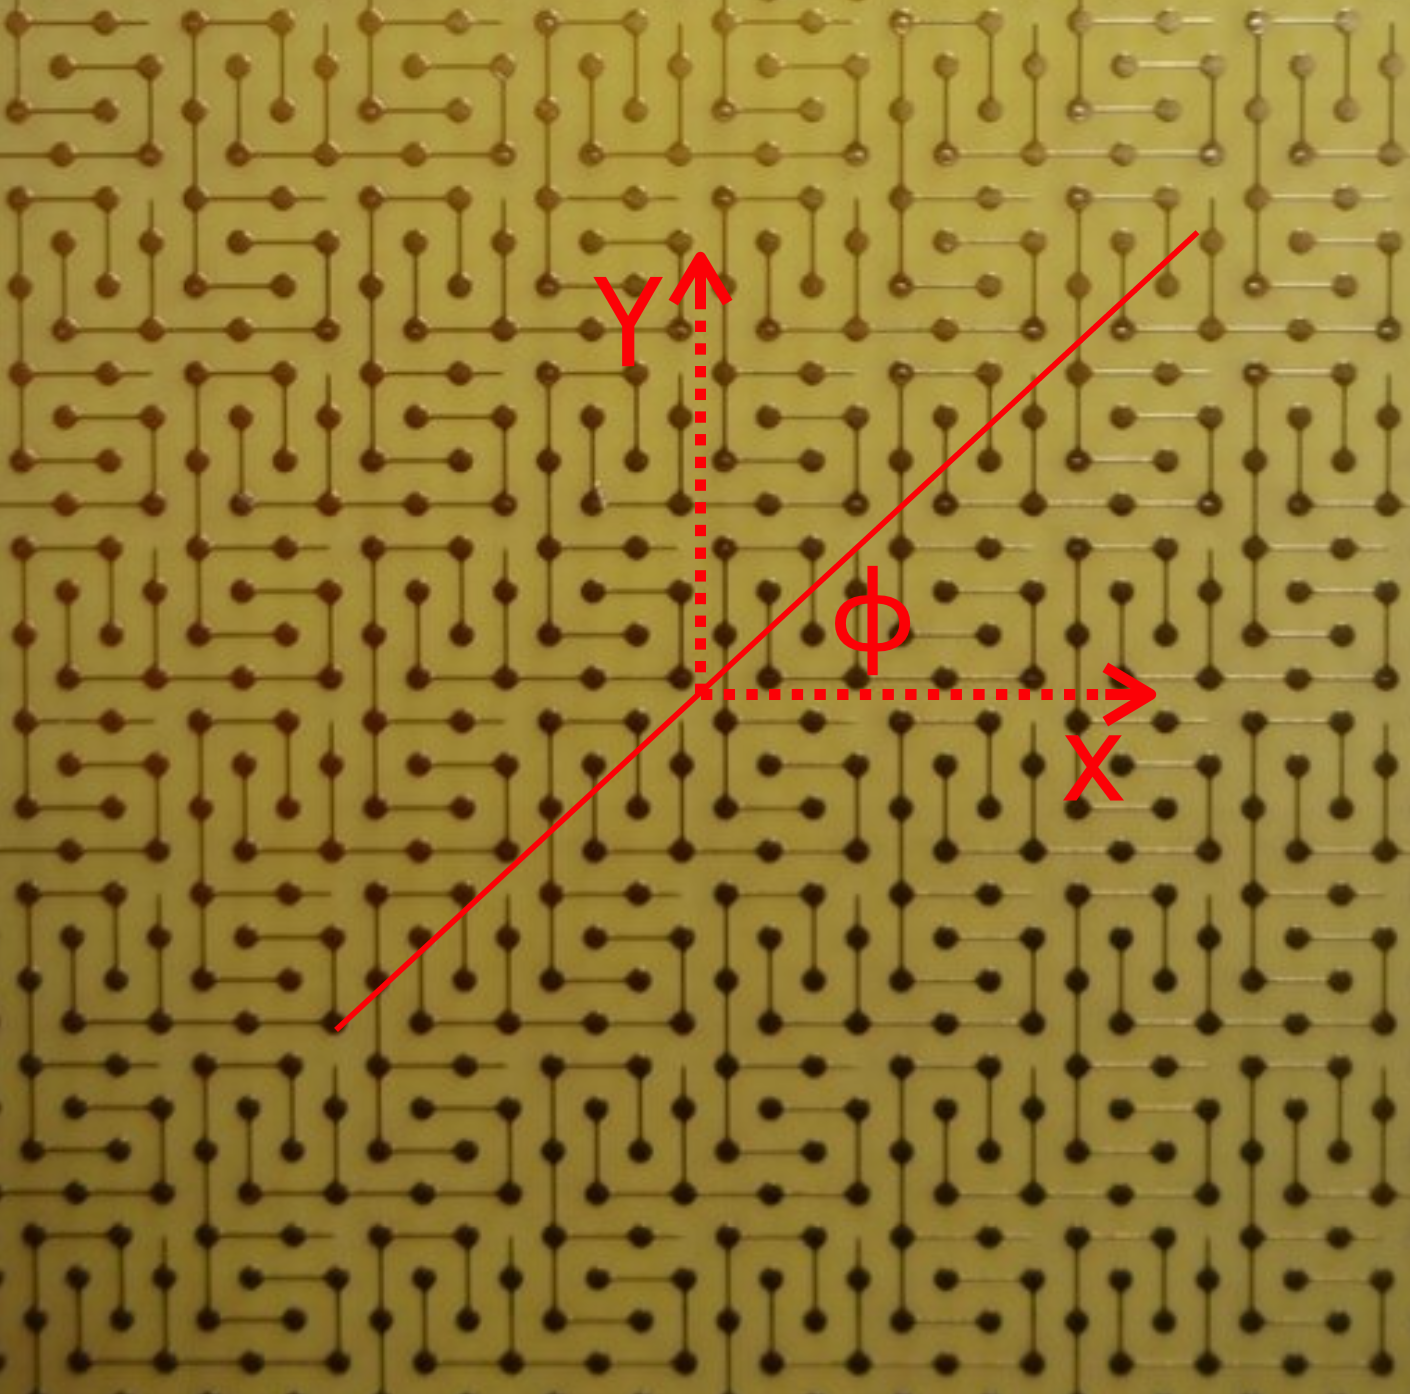
\includegraphics[scale=0.2]{anode_pcb} \hspace{0.2cm} 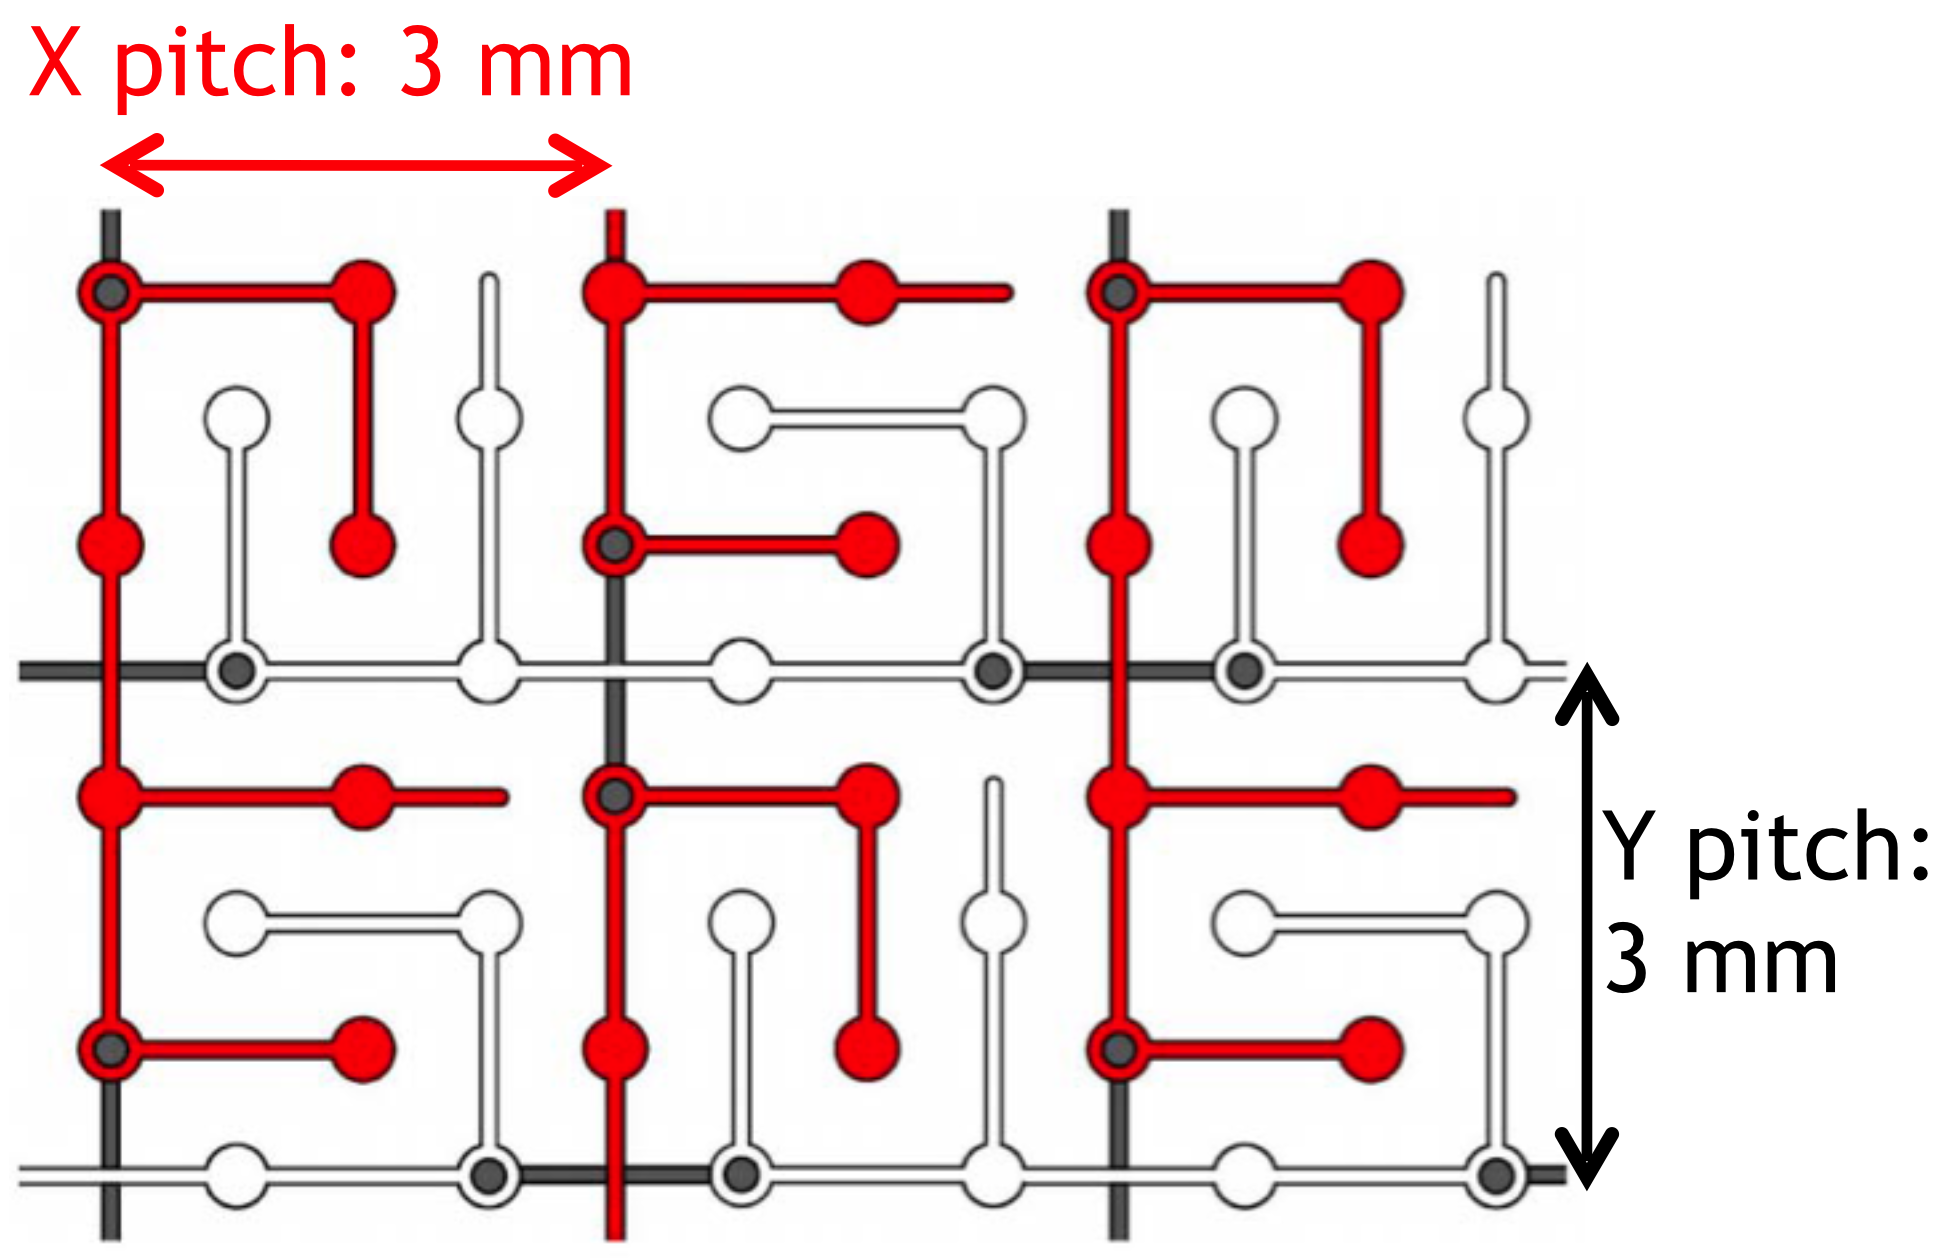
\includegraphics[scale=0.2]{anode_sch}
\end{cdrfigure}

As part of this optimization, the electrical capacitance of the
readout strips has been limited to only 150~pF/m, which translates
into an electronic noise of about $\sim$1000 electrons for 2-m readout
length.  Figure~\ref{fig:anode_res} (right) shows that the charge-sharing 
asymmetry between the two views is kept within 1\% . The two views can thus
be treated in a completely equivalent way from the
point of view of the reconstruction. The response in terms of the
charge collection per unit pathlength $\Delta Q/\Delta s$ is
independent of the charged-particle tracks' azimuthal angle $\phi$ (see
Figure~\ref{fig:anode_res} left and middle).
\begin{cdrfigure}[Charge deposition as function of track angle ]{anode_res}
{Charge deposition per unit of pathlength measured on LEM view 0 
($\Delta Q_0/\Delta s_0$) as a function  of the track angle $\phi$ (left) and 
projection of the  $\Delta Q_0/\Delta s_0$ distribution in three $\phi$ intervals (middle). 
The right plot  shows the distribution of the difference between the total charge  collected 
on both views normalized to their sum}
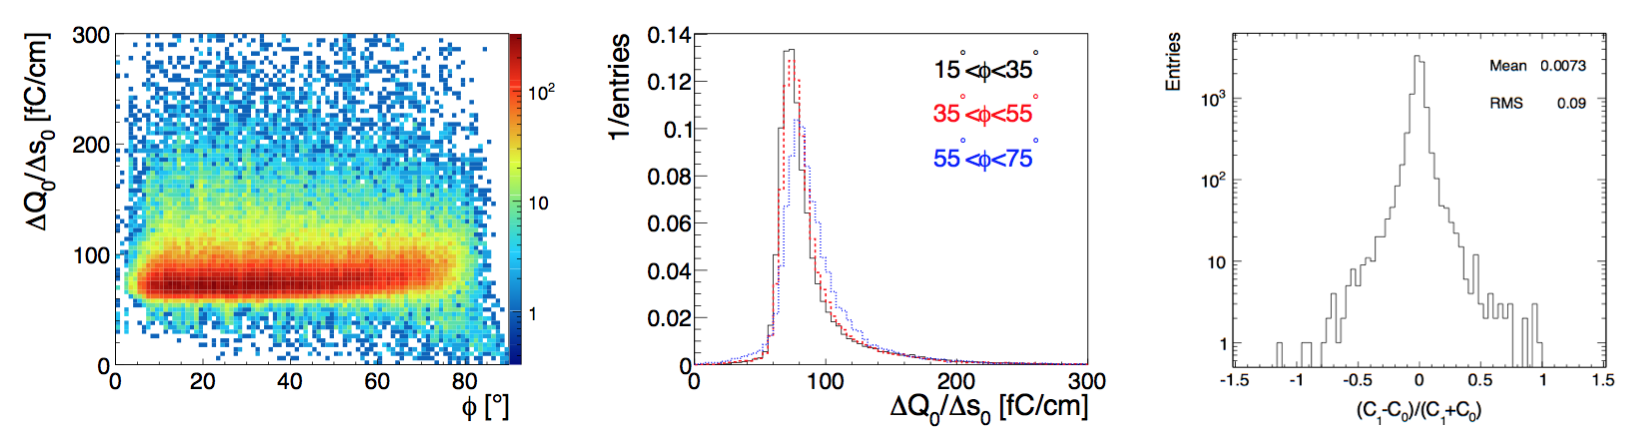
\includegraphics[width=.9\textwidth,scale=1]{anodeD_prop}
\end{cdrfigure}

\paragraph{The 0.5$\times$0.5~m$^2$ LEM:}
The LEM is built from a 1-mm thick copper-clad epoxy PCB with
mechanically drilled holes of 500~$\mu$m diameter surrounded by a
40-$\mu$m dielectric rim. The holes are arranged in a honeycomb
pattern with a pitch of 800~$\mu$m resulting in about 200 holes per cm$^2$
and $\cal O$(500,000) holes over the entire 50$\times$50~cm$^2$
area. The holes provide confinement for the UV photons produced
during the avalanche process and thus act as a mechanical quencher to
prevent photon feedback. This property makes the LEM suitable for
operation in ultra-pure argon vapor without the addition of a
quenching gas. The amplification of the drifting charges in pure argon
vapor at 87~K with LEMs has been extensively demonstrated on a chamber
with 10$\times$10~cm$^2$ area readout (see e.g.,
References~\cite{Badertscher:2008rf,Badertscher:2010fi}) as well as on a
larger device consisting of a $40\times80$~cm$^2$
readout\cite{Badertscher:2013wm}.  Both setups were successfully and stably operated 
%in a stable condition 
at constant gains of at least 15,
corresponding to S/N$\approx$60 for MIPs. Recent
studies~\cite{Cantini:2014xza} characterize systematically the impact
of the rim size, insulator thickness, hole diameter and hole layout on
10$\times$10~cm$^2$ area LEMs. The response in terms of maximal
reachable gain and influence on the collected charge uniformity as
well as the long-term stability of the gain has been thoroughly
compared for these different layouts. Some results are shown in
Figure~\ref{fig:LEM}.  Gains of almost 200 could be \fixme{could be or were?} reached and the
LEMs could be operated at stable gains of at least $\sim$15 after a
charging up period of about a day.
\begin{cdrfigure}[LEM performance vs geometry]{LEM}{Performance of the LEMs with different geometry parameters. Left: effective gain vs. LEM electric field; right: the stabilisations of the effective gain over time.}
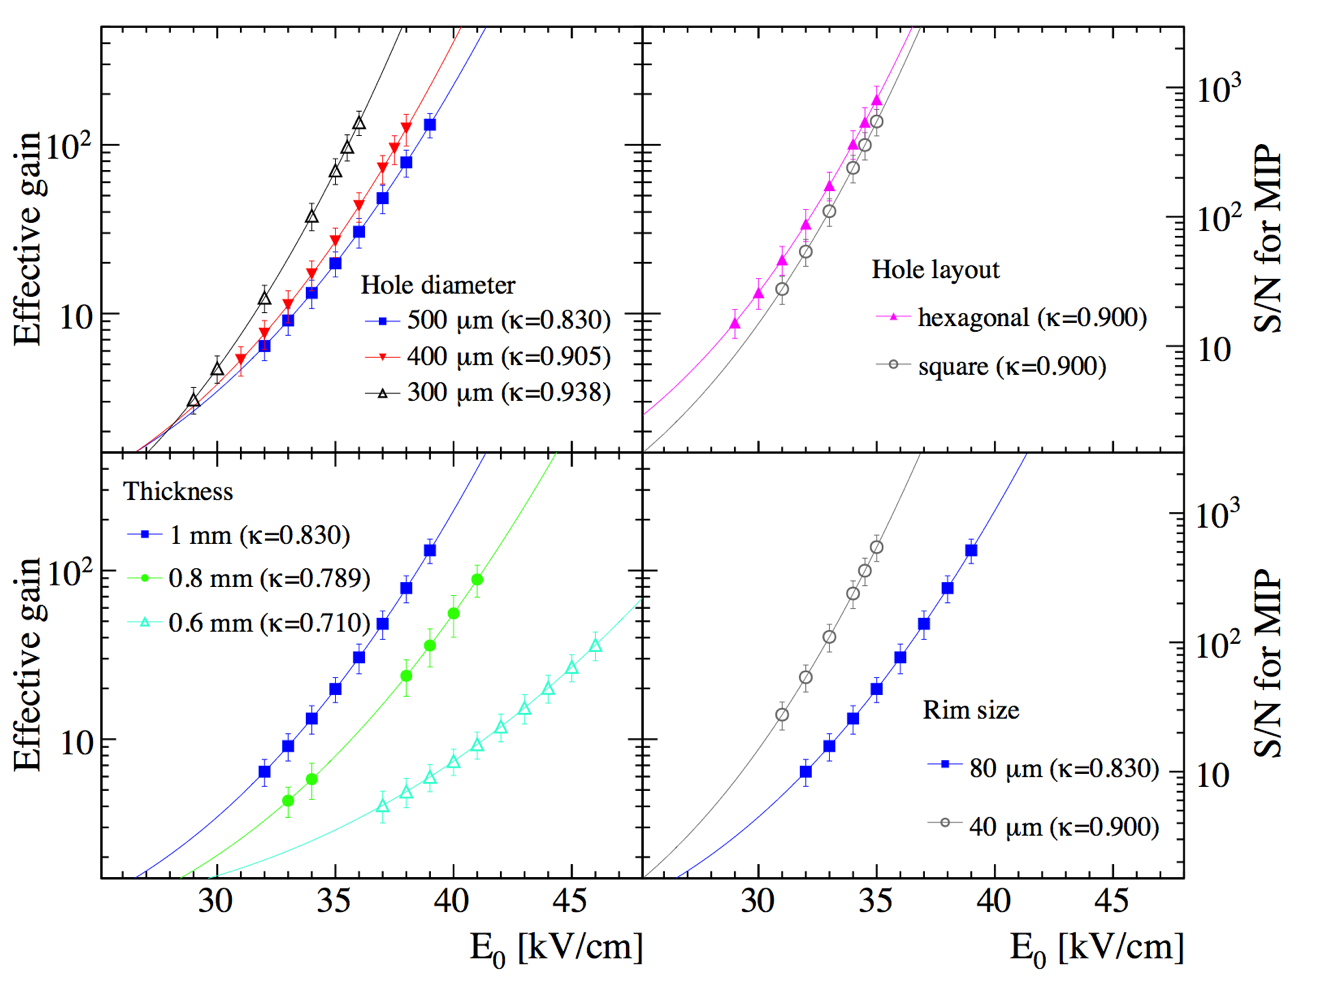
\includegraphics[scale=0.35]{4}
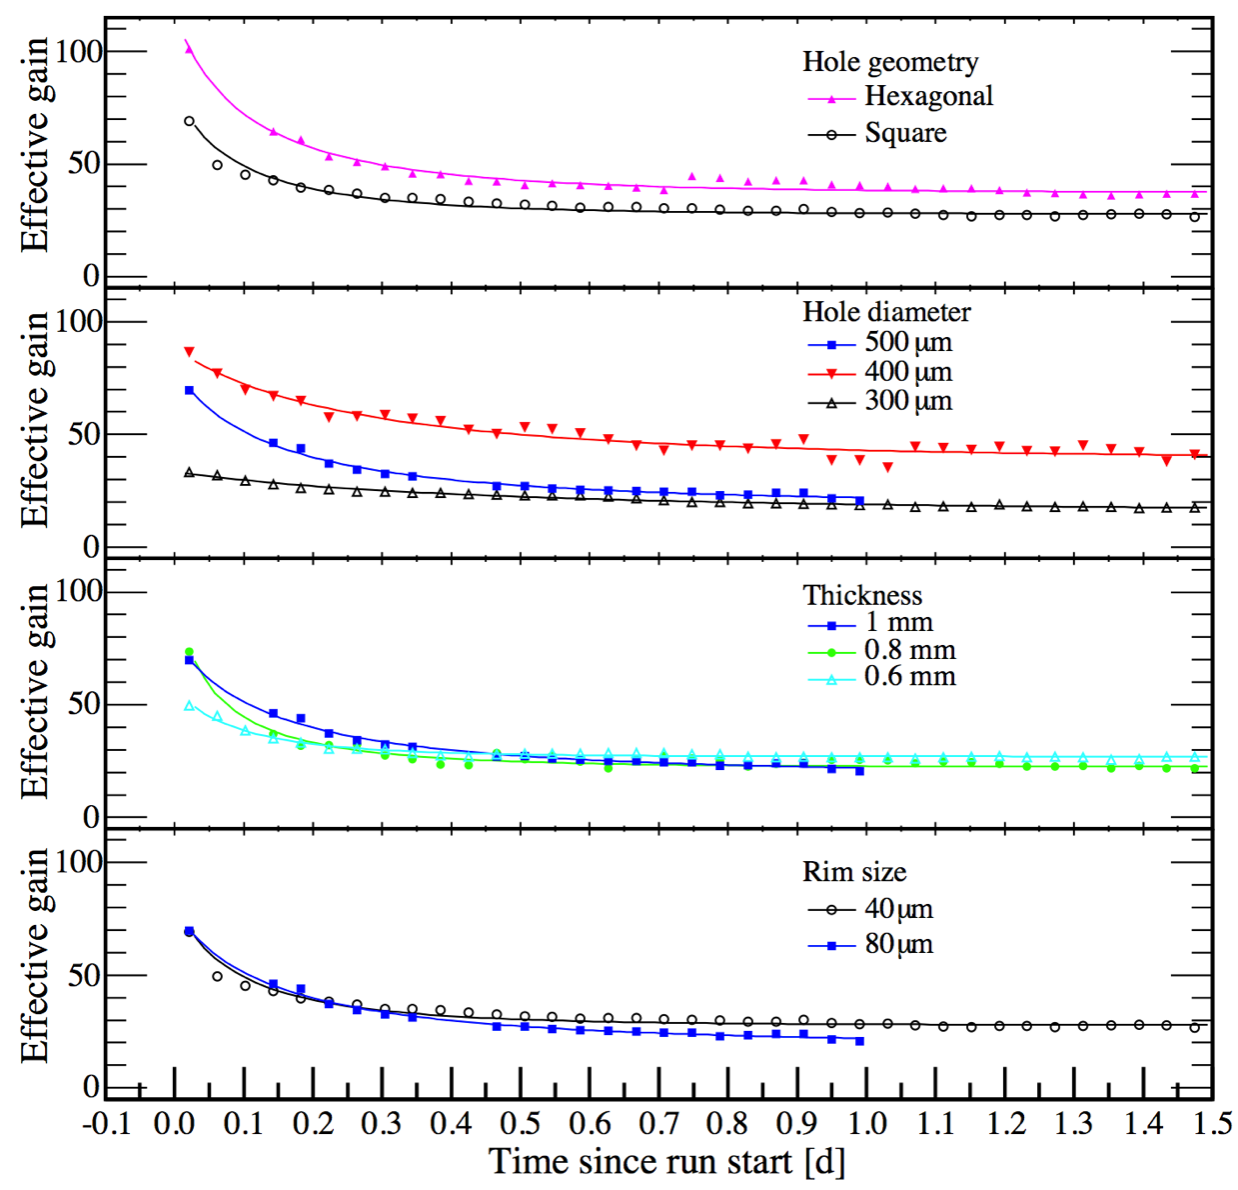
\includegraphics[scale=0.32]{3}
\end{cdrfigure}

\paragraph{LAS Assembly:}

Figure~\ref{fig:LEM_metro} shows the anode and LEM
sandwich.  They are fixed together with 29 M2 PEEK screws, each
containing a precisely machined 2-mm thick pillar to
guarantee a constant inter-stage distance between the entire
$50\times50$~cm$^2$ area. \fixme{between the entire area and what?}
 The dead zones caused by the supporting
pillars and the two HV pins on the LEMs are minimized and make up %correspond to
less than 0.5\% of the total area. The inter-stage distance between the
LEM and anode in the LAS has been measured at many points. The results
are shown in Figure~\ref{fig:LEM_metro} and are described
in~\cite{EDMS_metro_lem_anode}. They indicate that the planarity is
within the required tolerance of 2~mm$\pm$100~$\mu$m .
\begin{cdrfigure}[LEM/anode sandwich metrology]{LEM_metro}{Close up pictures of the LEM/anode sandwich. The two
       bottom figures show a the measurement at the CERN metrology lab
       and a histogram illustrating the measured gap between the LEM
       and anode in various points. As can be seen the distribution is
       centered on the nominal distance of 2~mm and has an RMS of
       about 100$\mu$m.}
     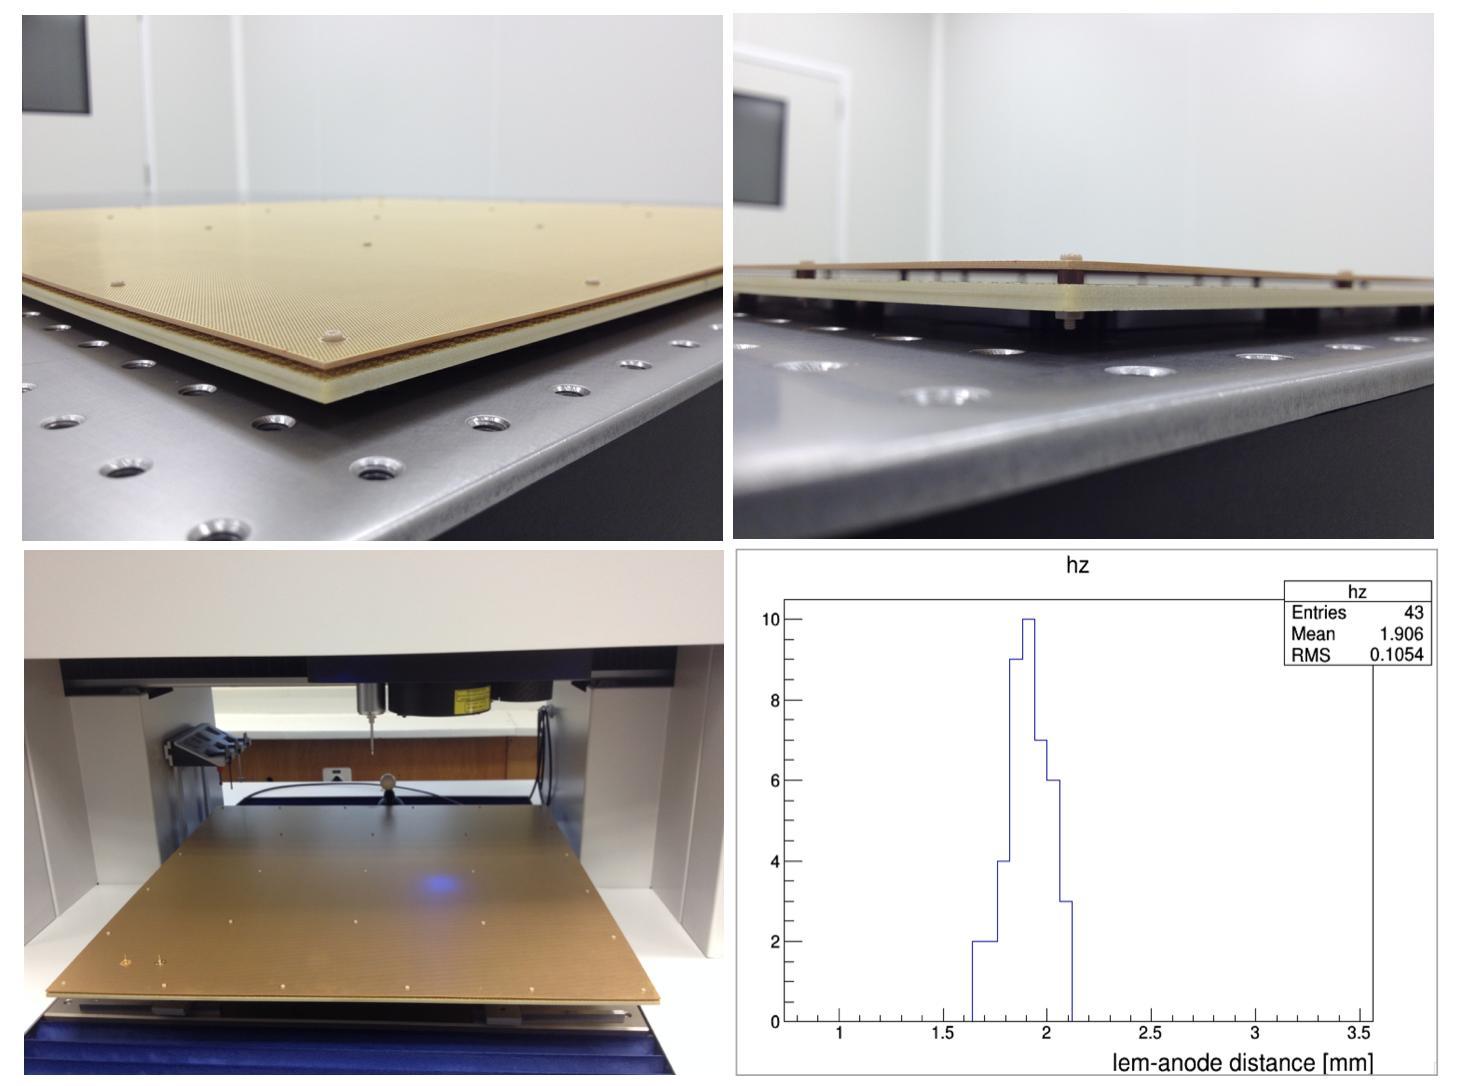
\includegraphics[width=.7\textwidth]{LEM_metro}
\end{cdrfigure}

The entire mounting sequence of the sandwich as well as that of the
different elements of the CRP are being addressed in the WA105
prototype detectors. An example of a sandwich assembly on a
$3\times1$~m$^2$ CRP is shown in Figure~\ref{fig:CRP_assembly}.
\begin{cdrfigure}[Pictures of the assembly of a $3\times1$m$^2$ CRP]{CRP_assembly}{Pictures of the assembly of a $3\times1$m$^2$ CRP}
     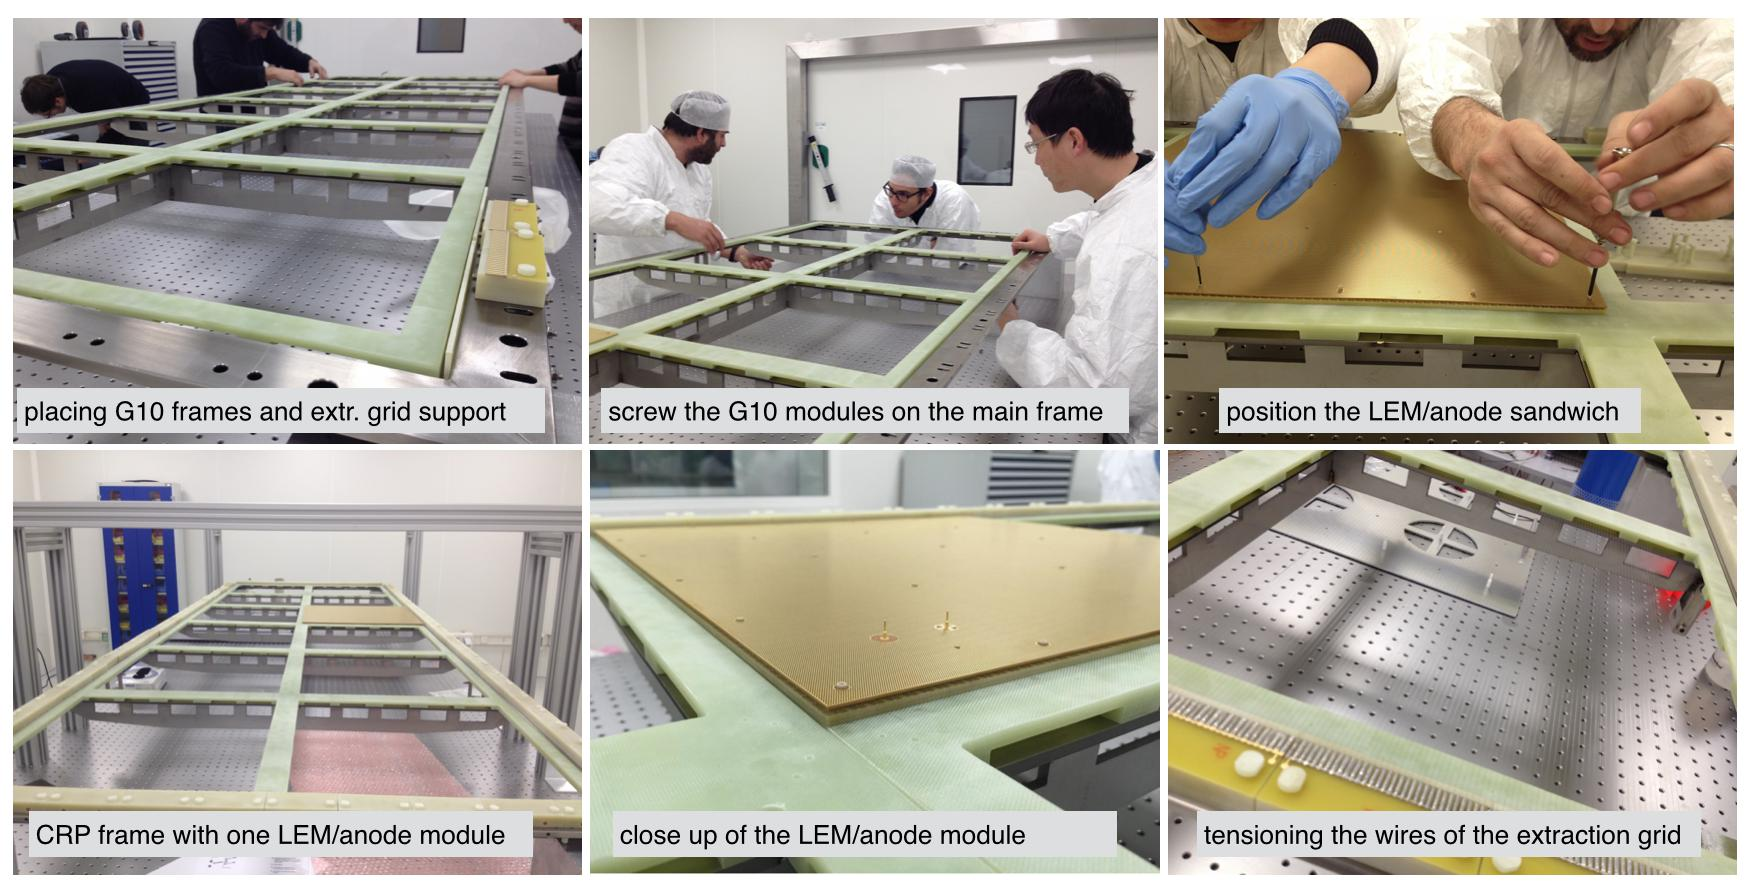
\includegraphics[width=\textwidth]{311_CRP_assembly}  
\end{cdrfigure}

